\begin{frame}[shrink=10]
    \frametitle{The FEniCS challenge!}
    \vspace{1em}
    \begin{columns}[c]
        \begin{column}{0.5\textwidth}
            Compute the Stokes flow around a swimming dolphin!
            \begin{itemize}
                \item Set a no-slip boundary condition on the upper and
                    lower channel walls and around the dolphin
                \item Set $u = (-\sin(\pi y),0)$ on the right inflow
                    boundary
                \item Impose $p=0$ on the left outflow boundary
                \item Implement a scheme based on Taylor--Hood elements
                \item Implement a scheme based on the stabilized
                $\PP_2/\,\PP_2$ elements with a stabilization parameter
                    $\beta$.  What happens if you reduce the size of
                    $\beta$?
            \end{itemize}
        \end{column}
        \begin{column}{0.5\textwidth}
            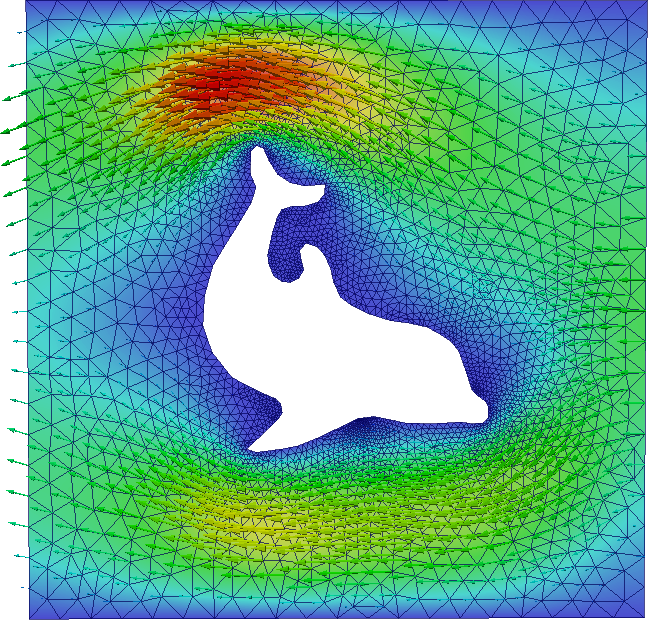
\includegraphics[width=1.0\textwidth]{png/stokes_dolphin_channel_u_alpha.png}
        \end{column}
    \end{columns}
    \begin{center}
    \end{center}
\end{frame}
